\subsection{多相机内外参联合标定}
\label{sec:camera_calib}

为了准确建模相机成像的光学过程,建立三维物体与二维照片之间的对应关系,需要对相机的内参和外参进行标定。
即准确测量采集过程中用到的每一台相机的内参和外参。
其中,内参包括相机的焦距、光心坐标、畸变参数等,
外参则包括不同相机之间的相对位置和姿态。

本方案选用的相机模型是针孔相机模型,这也是在实验中采用的相机所遵循的模型。
由于本实验中相机畸变较小,简单起见,本文选用了OpenCV中默认的径向和切向相机畸变模型\footnote{\url{https://docs.opencv.org/4.7.0/d4/d94/tutorial_camera_calibration.html}}。
更正式地,假设共有$N$个相机,对于第$i$个相机($i=1,2,\cdots,N$),
内参标定的目标是求解该相机的
焦距$f_x^{(i)},f_y^{(i)}$、
光心坐标$c_x^{(i)},c_y^{(i)}$、
畸变参数$k_1^{(i)},k_2^{(i)},k_3^{(i)},p_1^{(i)},p_2^{(i)}$;
外参标定的目标则是求解该相机在世界坐标系下的
位置$\mathbf{t}^{(i)}=\left(x^{(i)},y^{(i)},z^{(i)}\right)$
和姿态$\mathbf{r}^{(i)}$。
其中$\mathbf{r}\in \mathbb{R}^3$为表示三维旋转群$\mathrm{SO(3)}$的的指数映射向量,
其表示轴为$\mathbf{r}$,角度为$\left\| \mathbf{r}\right\|$的旋转。
世界坐标系的选取是任意的,因此在相机标定阶段,不失一般性地,我们选择第一次快门触发时的标定板坐标系为世界坐标系。
\def\camparam{\delta}
综上,在标定过程中共需要求解$N\times 15$个参数,记为$\camparam$。
在该模型下,对于任意在世界坐标系下的点$\mathbf{X}\in \mathbb{R}^3$,其在第$i$个相机的成像平面的投影点$\mathbf{x}^{(i)}$的计算过程可称为相机投影,记为$\mathbf{x}^{(i)}=\pi(\camparam_i, \mathbf{X})$。
$\pi$的形式化定义可参见附录\ref{app:camera_model}。

为了解算上述模型中的参数,通常需要使用待标定的相机对一类特殊的物体进行拍摄,称为标定物体。
它们的特点是通常有一些在照片中容易被计算机视觉算法识别的特征点,且这些点容易在不同相机拍摄的照片间进行匹配。
这类物体通常为标定板,即印有棋盘格、二维码、圆形或者其他易于识别的图案的硬质平面板子。
也有一些方法\cite{colmap}使用SIFT等特征点算法来自动从任意被拍摄物体上提取和匹配特征点。但这种方法匹配成功率稍低,且忽略了物体反射光线的各向异性,因此可能会带来一些误差。

\paragraph{数据采集}
\begin{figure}
    \centering
    \begin{minipage}{0.5\textwidth}
        \centering
        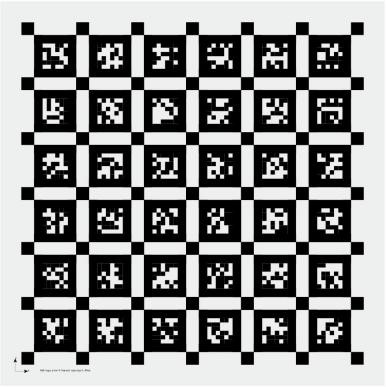
\includegraphics[height=6cm]{figures/april_board}
        \captionof{figure}{April Board上的二维码和棋盘格图案}
        \label{fig:april_board}
    \end{minipage}%
    \begin{minipage}{0.5\textwidth}
        \centering
        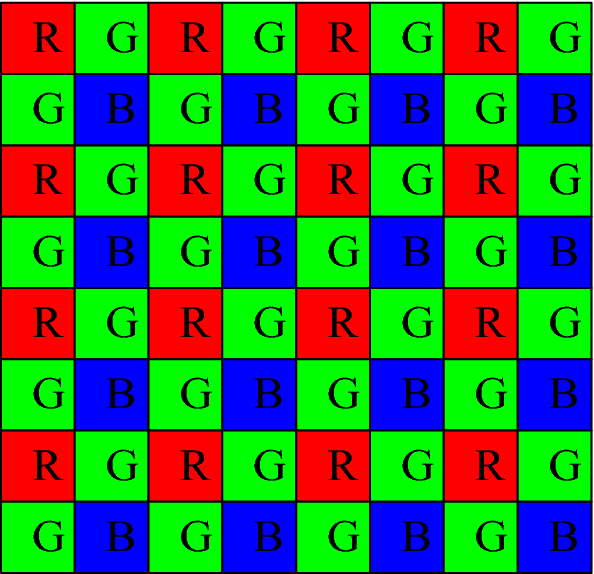
\includegraphics[height=6cm]{figures/bayer}
        \captionof{figure}{Bayer格式照片示意图}
        \label{fig:bayer}
    \end{minipage}%
\end{figure}

本方案中使用的标定物体为April Board,即印有二维码和棋盘格组成的图案的标定板,如图\ref{fig:april_board}所示。
该标定板的尺寸为$800 \times 800$毫米,每个二维码的边长为$88$毫米。
该图案中棋盘格的十字角点可由算法精确完成亚像素级定位,而密集的二维码则便于在不同照片中便捷地匹配角点。
其采用了玻璃基板,以保证标定板的刚性和平整度;
同时采用了氧化铝表面,使标定板表面无明显镜面反射光斑,确保标定板在不同光照条件下的可靠性。

在拍摄标定物体时,需要注意保持相机处于手动对焦模式,关闭光学防抖,以防止其内外参意外发生变化。
并使用前述(第\ref{sec:passive_sync}节)被动相机同步装置同时触发所有相机进行拍摄。转动标定板,重复触发快门15-20次。

\paragraph{相机标定优化目标}
\def\cornerpix{\mathbf{o}}
\def\cornerboard{\mathbf{w}}
本方案中的相机标定算法接收照片中的特征点坐标作为输入,求解上述相机模型中的参数$\camparam$。
正式地,假设共触发了$M$次快门,标定板中共有$K=144$个角点,算法的输入包括第$i$个相机在第$j$次触发快门时拍摄的第$k$个角点($j = 1,2,\cdots,M$、$k = 1,2,\cdots,K$)在像素坐标系中的坐标$\cornerpix_{i,j,k}\in \mathbb{R}^2$;
以及角点在标定板坐标系中的坐标$\cornerboard_k\in \mathbb{R}^3$。
由于每次触发快门时标定板都由人工转动,因此其在世界坐标系中的位置也是未知的,故将第$j$次快门时标定板坐标系到世界坐标系的刚体变换$T_{j}(\cdot)\in \mathrm{SE(3)}$也做为未知量。
其中固定$T_{1}$为幺元,即$T_{1}(X) = X$,以确定世界坐标系的位置。
则本文中的相机标定问题可以表示为以下最小二乘优化问题:
\begin{equation}
    \label{eq:calib_opt}
    \argmin_{\camparam,T} \sum_{i,j,k} \left\| \cornerpix_{i,j,k} - \pi\left(\camparam_i, T_j(\cornerboard_k)\right) \right\|_2^2
    \text{。}
\end{equation}
为实现该目标,首先需要在每张照片中识别角点,并以亚像素级精度精确定位其坐标$\cornerpix_{i,j,k}$。
本节后续将介绍角点的识别、精确定位,模型初始化及上述优化问题的具体求解方法。

\paragraph{角点识别}为识别标定板中可供拟合的角点,本文首先识别照片中的二维码,并将二维码的四个角作为角点的候选点。
本文所用标定板上的二维码为AprilTag,本文实现的识别算法也是基于其开源的方法\cite{AprilTag}。
该算法是一个自下而上的算法,它首先从照片中识别直线段,然后将直线段组合成四边形,最后试图将四边形区域识别为二维码。得益于二维码的纠错功能,虽然该方法召回率稍低,但查准率非常高。同时二维码中存储的信息可用于角点在不同照片中的匹配。

本文所实现的版本的输入为相机拍摄的,原始Bayer格式的照片,该照片是单通道图像,其中RGB像素排列如图\ref{fig:bayer}所示,每$2\times 2$个像素中包括一个红色像素、两个绿色像素和一个蓝色像素。每种像素的传感器前带有滤光片,仅允许特定波长的光被传感器捕获。因此,Bayer格式的照片中,每个像素的值即为该像素对应的颜色通道的光照强度。
为了减少冗余的数据处理流程,并保持全流程的可解释性以准确控制误差,本方案直接使用了原始照片,而没有使用常见的相机后处理后输出的RGB格式图像。

由于我们所拍摄的照片分辨率远超二维码识别所需,因此本文先对照片进行降采样。
其具体方法是,首先在每4个像素中仅取一个绿色像素,以排除颜色对二维码识别的影响;
再进行5倍平均池化,即最终降采样后的图像长宽为原图的$1/10$。
以此降低算法耗时并大大降低照片中的噪声等级,提升算法的鲁棒性。
在低分辨率的图像上完成二维码识别后,二维码的四个角的坐标将被重新映射回完整分辨率的像素坐标,以初始化后续的精确定位步骤。

% 本文使用的相机拍摄的原始照片分辨率高,可达$5472\times 3648$;
% 且宽容度高,其量化后的亮度可达约13000级,相比普通JPG照片仅有256级。
% 因此,本文在\cite{AprilTag}的基础上,设计了尺度、亮度无关的直线段识别算法,使其更加鲁棒,并减少算法超参数调节的麻烦。
% \TODO{尺度、亮度无关的直线段识别算法}

\paragraph{角点精确定位}在上一步识别出角点后,该步骤依据角点周围的像素值,获取这些角点尽可能精确的像素坐标$\cornerpix_{i,j,k}$,以保证标定的精度。
该步骤的难点在于,算法需要对失焦造成的模糊、成像过程中的噪声等因素足够鲁棒,并达到亚像素级的精度。
本文采用的算法为\citet{ROCHADE}提出的精确角点定位算法,其基本思想为:
使用一个二维多项式函数对角点周围的像素进行拟合,然后以该多项式函数的鞍点作为该角点的精确像素坐标。

具体地,本文首先需要从照片原始数据获取单通道灰度图。
该灰度图在标定板区域的每个像素值应表征标定板表面反射的总光强,而不与颜色有关。
为此,需要对红色、蓝色像素值进行缩放,使其与绿色像素匹配(相当于相机的白平衡操作),其缩放系数与环境光照、标定板材质等有关。
本文假设标定板任意位置反射的光线的波长分布是均匀的。
因此,本文首先对上一步求得的二维码区域求凸包,以定位照片中的标定板,并调整缩放系数以使该区域中不同颜色像素的均值相等。
然后,对该图使用半径为$r$的圆锥形kernel进行滤波,以使像素值平滑,从而能更好地被多项式函数拟合。
最后,以角点的当前估计位置为中心,使用二阶二维多项式函数对周围的$(2r+1) \times (2r+1)$个像素进行最小二乘拟合:
\begin{equation}
    \label{eq:poly}
    \hat{a} = \argmin_{a} \sum_{x,y} \left(\bar{\mathcal{I}}(x, y) - (a_0 x^2 + a_1 y^2 + a_2 xy + a_3 x + a_4 y + a_5)\right)^2
    \text{,}
\end{equation}
其中,$\bar{\mathcal{I}}$为滤波后的灰度图。
在实现上,本方案直接使用解析公式求解该线性最小二乘问题。并求该二维多项式函数的鞍点作为该角点新的估计位置:
\begin{equation}
    \label{eq:subpixel}
    \begin{cases}
        x' &= -\dfrac{\hat{a}_2 \hat{a}_4 - 2 \hat{a}_1 \hat{a}_3}{\Delta} \\
        y' &= -\dfrac{\hat{a}_2 \hat{a}_3 - 2 \hat{a}_0 \hat{a}_4}{\Delta}
    \end{cases},\quad
    \Delta = 4 \hat{a}_0 \hat{a}_1 - \hat{a}_2^2
    \text{,}
\end{equation}
并如此迭代,直到角点的估计位置收敛,该收敛的位置即为$\cornerpix$。
在此过程中,若估计位置超出了图像范围,或$\Delta < 0$,则将该角点排除。
$\Delta < 0$的原因通常是该角点被其他物体遮挡,或者受到其他物体投下的阴影影响。

\def\cornerincode{\hat{\cornerpix}}
在该算法中,$r$的选取可能对结果产生较大影响。较大的$r$将能利用照片中更多像素的信息,从而对噪声更加鲁棒,但也不能过大,否则周边的二维码,或相邻的其他角点等无关信息将影响拟合结果。为此,本文依据上一步识别到的二维码的尺寸以自适应地选择$r$。令$\cornerincode_{i,j}$为照片中第$i$个二维码的第$j$个角点的估计位置,$j\in\{0,1,2,3\}$,以顺时针方向排列,则$r$的选取为:
\begin{equation}
    \label{eq:r}
    \begin{aligned}
        l_{i,\textrm{edge}} & = \min_j\left(\|\cornerincode_{i,j} - \cornerincode_{i,j+1\bmod 4}\|\right)\text{,} \\
        l_{i,\textrm{diag}} & = \min\left(\|\cornerincode_{i,0} - \cornerincode_{i,2}\|, \|\cornerincode_{i,1} - \cornerincode_{i,3}\|\right)\text{,} \\
        r & = \min_i\left\{0.07 l_{i,\textrm{edge}}, 0.05 l_{i,\textrm{diag}}\right\}\text{。}
    \end{aligned}
\end{equation}

\paragraph{多相机内参标定与外参传递}
获得角点精确位置后,本文分为两个阶段求解公式\eqref{eq:calib_opt}。
在第一阶段,本文将对每台相机分别进行标定,获得各相机的内参初始化值
并估计标定版在每次触发快门时与各台相机的相对位置。
具体地,本文依据相机和镜头厂商提供的传感器尺寸、图像分辨率、镜头焦距初始化相机内参$f$、$c$。
然后调用OpenCV中单台相机标定的算法,使用PnP算法求解标定板在每次触发快门时与相机的相对位置$T_{i,j}$;
并使用Levenberg-Marquardt算法对这些参数进行调整。

由于不同相机的同一次快门的触发是严格同步的,因此可以认为若不同相机在同一次快门的触发时,拍摄到的标定板在世界坐标系中的位置是相同的。
据此可将每台相机,以及每次快门触发作为节点,构建二部图,图中的边表示该相机在该次快门中拍摄到了标定板。
若该二部图是连通图,则可迭代地将所有相机、所有快门触发中的标定板的位置传递到世界坐标系中,
如算法\ref{alg:calib_init}所示。
并最终获得$\delta$和$T$中所有参数的初始化值。

\begin{algorithm}[t]
    \caption{外参传递}
    \label{alg:calib_init}
    \begin{algorithmic}[1]
        \Require 连通二部图$(V,E)$;第$j$次快门时标定版坐标系到相机$i$坐标系的刚体变换$\hat{T}_{i,j}\in SE(3),(i,j)\in E$
        \Procedure{外参传递}{$V,E,\hat{T}_{i,j}$}
            \State $C \gets \emptyset$\Comment{已传递的相机集合}
            \State $T_{1} \gets \mathbf{I}$\Comment{以第$1$次快门时标定版坐标系作为世界坐标系}
            \State $S \gets \{1\}$\Comment{已传递的快门触发集合}

            \While{$C \cup S \neq V$}
                \State $i \gets \forall i\in V| i\notin C, \exists j\in S| (i,j)\in E$
                    \Comment{选择与已知位置的标定板相邻的相机}
                \State $U_{i} \gets T_{j}\hat{T}_{i,j}^{-1}$
                    \Comment{相机$i$到世界坐标系的变换}
                \State $C \gets C \cup \{i\}$
                \ForAll{$j | (i,j)\in E, j\notin S$}
                    \State $T_{j} \gets U_{i}\hat{T}_{i,j}$
                        \Comment{第$j$次快门时标定版到世界坐标系的变换}
                \EndFor
                \State $S \gets S \cup \{j\in V| (i,j)\in E\}$
            \EndWhile
            \State \Return $U, T$
        \EndProcedure
    \end{algorithmic}
\end{algorithm}

\paragraph{集束调整}在第二阶段,本文将对所有相机进行集束调整,即直接使用公式\eqref{eq:calib_opt}中的目标函数,在上一阶段的初始化值的基础上,同时优化模型中的所有参数。
具体地,本文使用了Levenberg-Marquardt算法\cite{lm},对目标函数进行优化求解。
并手动实现了公式\eqref{eq:calib_opt}的雅克比矩阵的解析求解算法,以提升算法的速度和收敛精度。

然后,排除掉误差较大的角点,再次重复上述优化过程,并如此迭代数次,每次使用更严格的误差阈值进行排除。
这些误差较大的角点通常是由于角点定位不准确造成的,因此,将其排除后可以提高标定的精度。
该优化过程最终得到的相机参数$\camparam$即为所求的最终的相机标定结果。
